\documentclass[a4paper]{article}

%% Language and font encodings
\usepackage[english]{babel}
\usepackage[utf8]{inputenc}
\usepackage[T1]{fontenc}
\usepackage[backend=bibtex,style=ieee]{biblatex}

%% Sets page size and margins
\usepackage[a4paper,top=3cm,bottom=2cm,left=3cm,right=3cm,marginparwidth=1.75cm]{geometry}

%% Useful packages
\usepackage{amsmath}
\usepackage{graphicx}
\usepackage[colorinlistoftodos]{todonotes}
\usepackage[colorlinks=true, allcolors=blue]{hyperref}
\usepackage{wrapfig}

\hypersetup{
	urlcolor= blue,  %couleur des hyperliens
	linkcolor= black, %couleur des liens internes
}


\newcommand{\HRule}{\rule{\linewidth}{0.5mm}} % Defines a new command for the horizontal lines, change thickness here


\title{Recherche Bibliographique}
\author{Andres Julien, Taylor Thomas}
\date{}

%% Citations

\bibliography{bib/kilobots} 
\nocite{*}

\begin{document}

\begin{titlepage}
\center


\includegraphics{incl/logo_sorbonne}\\[1cm] 

\HRule \\[0.4cm]
{ \huge \bfseries Robotique en essaim }\\
{ \huge \bfseries Recherche Bibliographique}\\[0.4cm] % Title of your document
\HRule \\[1.5cm]



Julien \textsc{Andres}\\ % Your name
Thomas \textsc{Taylor}\\[3cm]

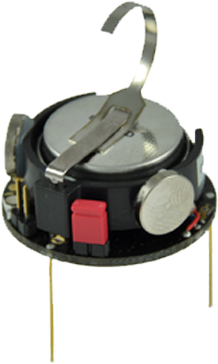
\includegraphics[width=4cm]{incl/Kilobots.png}



\end{titlepage}

\newpage
\section{Introduction}

La robotique en essaim est une branche de la robotique qui étudie la coordination de grandes populations de robots à comportements simples pour exécuter une tâche complexe. Elle s'inspire des colonies d'insectes sociaux, comme la fourmi ou l'abeille, qui peuvent réaliser des tâches en groupe, alors qu'un individu seul en est incapable. \\ Pour étudier la robotique en essaim, nous disposons d'une flotte de 100 Kilobots, un robot de 2 cm de diamètre pouvant communiquer via infrarouge et se déplacer à l'aide de deux moteurs à vibrations. Le but de ce projet est d'étudier plusieurs comportements fondamentaux tels que la couverture et l'agrégation et de les adapter aux Kilobots. Nous avons ensuite implémenté un algorithme d'apprentissage dit d'\textit{embodied evolution} dirigé par la pression environnementale, afin d'observer la dynamique adaptative de l'essaim en fonction de la structure de l'environnement.

\section{Mots clés retenus}

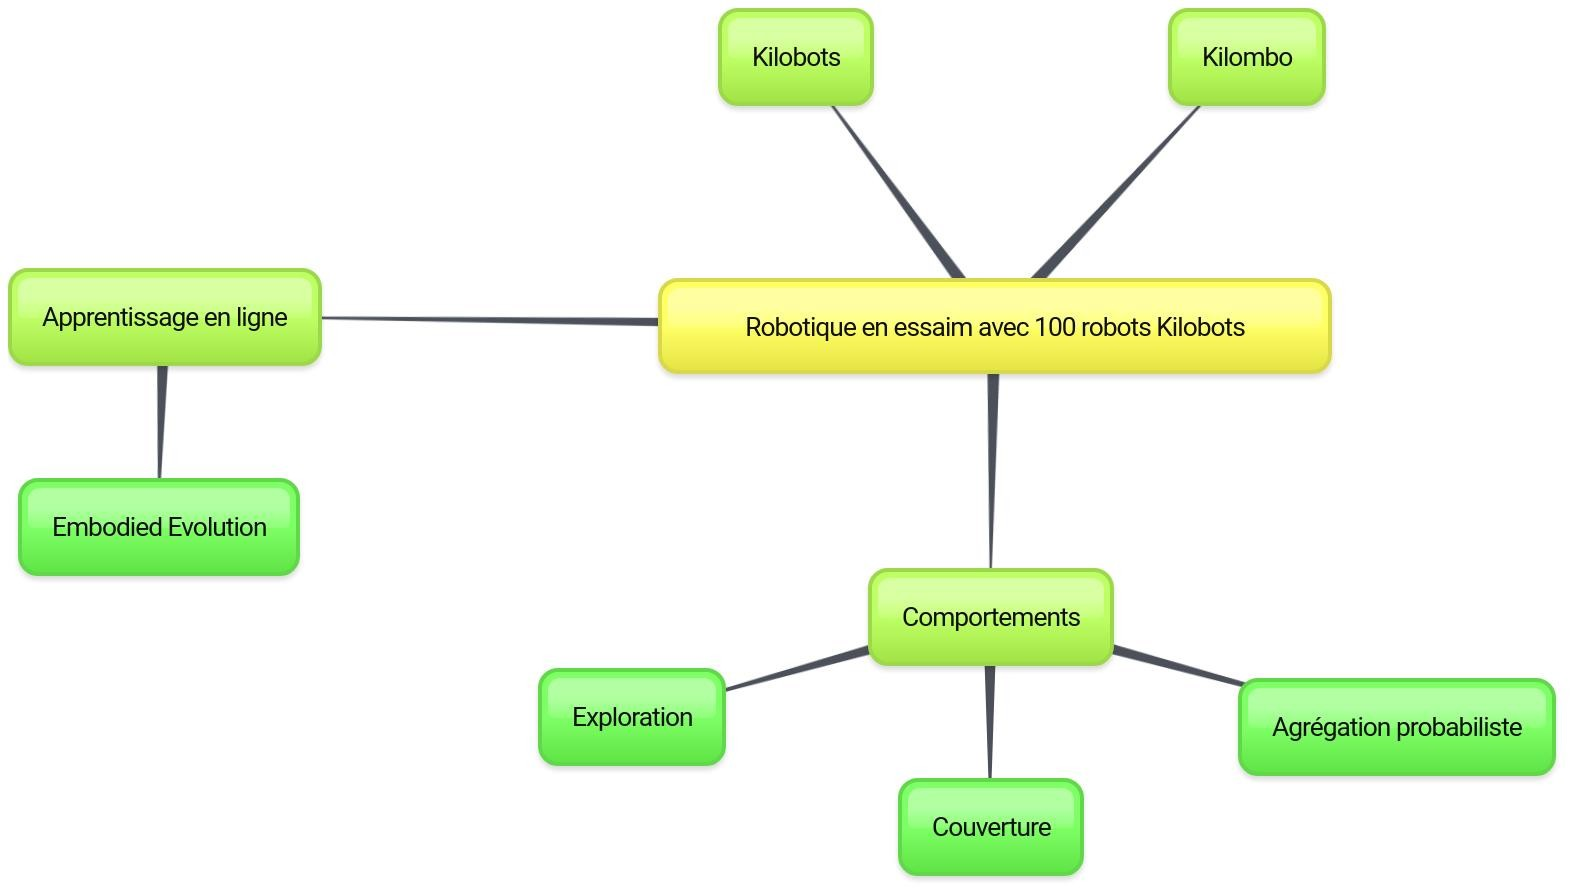
\includegraphics[width=15cm]{incl/carte_heuristique.jpg}

\section{Descriptif de la recherche documentaire}

Dans un premier temps, nous nous sommes documentés sur le fonctionnement des kilobots et du simulateur utilisé par le groupe précédent. Nous avons donc consulté les articles fournis par notre encadrant, rédigés par les chercheurs à l'origine du Kilobot.
Avec les références fournies dans ces articles, nous avons appliqué la méthode de recherche par rebond pour affiner notre bibliographie afin de sélectionner des sources traitant des comportements à étudier. \\ Cependant, pour éviter de se restreindre à ces seuls articles, nous avons étendu notre recherche grâce à Google Scholar, qui est un moyen simple de se documenter et de rassembler des sources sur un sujet à ressort scientifique. Sur les pages utilisateurs, nous avons pu identifier d'autres chercheurs ayant rédigé des articles concernant notre sujet grâce à la section co-auteurs. Le nombre de citations affiché sur ces pages permettent aussi de vérifier la fiabilité et la pertinence de la source. Alors que la recherche par auteur s'est montrée plus fructueuse sur Google Scholar, en cherchant les mots-clés en rapport à notre projet, la base de données IEEE accessible grâce à la BUMPC, nous a permis un grand nombre d'articles sur la robotique en essaim.

\section{Bibliographie produite}

\printbibliography

\section{Analyse des sources}

\subsection{Probabilistic aggregation strategies in swarm robotic systems}

Cette source est l’une des premières étudiée lors de la première recherche de comportements à étudier. Découverte à l’aide de Google Scholar, elle fut consultée de nombreuses fois à l’aide de IEEE. Elle propose une approcheprobabiliste pour construire une agrégation entre les robots. Référencée dans plusieurs articles
étudiés par la suite, cette source s’est avérée fiable. Notre principal algorithme d’agrégation est
basé sur celui présenté dans cet article.

\subsection{Environment-Driven Embodied Evolution in a Population of Autonomous Agents}

Cette source nous a directement été fournie par notre encadrant, il en est le principal auteur. C'est grâce à cet article que nous avons pu implémenter notre algorithme d'embodied evolution, mEDEA. Elle est citée à de nombreuses reprises dans d'autres articles consultés qui traitent du sujet.

\subsection{Kilobot: A low cost scalable robot system for collective behaviors}

L'article \textit{Kilobot: A low cost scalable robot system for collective behaviors} présente le Kilobot, robot utilisé durant toute la durée du projet. Cet article nous a permis en premier lieu de découvrir ses caractéristiques ainsi que des comportements de bases développés sur ces robots (notamment la self-assembly), grâce aux nombreux articles auquel cette source fait référence. Il nous a permis d'obtenir une vue d'ensemble sur notre sujet et a constitué d'un très bon point de départ pour notre recherche bibliographique. Il est rédigé par les créateurs du Kilobot, ce qui en fait une source assurément fiable.

\end{document}